%%%%%%%%%%%%%%%%%%%%%%%%%%%%%%%%%%%%%%%%%%%%%%%%%%%
%
%  New template code for TAMU Theses and Dissertations starting Fall 2012.  
%  For more info about this template or the 
%  TAMU LaTeX User's Group, see http://www.howdy.me/.
%
%  Author: Wendy Lynn Turner 
%	 Version 1.0 
%  Last updated 8/5/2012
%
%%%%%%%%%%%%%%%%%%%%%%%%%%%%%%%%%%%%%%%%%%%%%%%%%%%

%%%%%%%%%%%%%%%%%%%%%%%%%%%%%%%%%%%%%%%%%%%%%%%%%%%%%%%%%%%%%%%%%%%%%%
%%                           SECTION I
%%%%%%%%%%%%%%%%%%%%%%%%%%%%%%%%%%%%%%%%%%%%%%%%%%%%%%%%%%%%%%%%%%%%%
%
\chapter{\uppercase {Hyperbolic conservation laws}}\label{chap:theory_chp1}
%
In this chapter, some key properties of hyperbolic conservation laws are recalled. The objective is to introduce the reader to the notion of shocks, weak solutions, and entropy conditions by first studying a simple hyperbolic scalar equation. The mathematical properties of the hyperbolic scalar equation are studied, including the derivation of the Jacobian eigenvalues and the characteristic equations. Then, we explain how a shock is formed which leads to a discussion of solution non-uniqueness and weak solutions. We explained how the entropy condition is used to ensure uniqueness of the weak solution and, finally, we discuss convergence of the numerical solution to the physical one. In the last section of this chapter, the notions introduced for the hyperbolic scalar equation are generalized to hyperbolic systems of equations.

%%%%%%%%%%%%%%%%%%%%
\section{Hyperbolic scalar equations}\label{sec:hyp_scalar_sct1b}
%%%%%%%%%%%%%%%%%%%%

The study of a hyperbolic scalar equation is first given in order to provide the reader with an understanding of the  mathematical properties that are needed to aid in the comprehension of shock formation, among other topics.

%=============================
\subsection{Eigenvalue and characteristic curves}\label{sec:mat_ppr_sct1b}
%=============================
Consider a simple hyperbolic scalar equation with initial and boundary conditions to form what is called an \emph{Initial Boundary Value Problem} (IBVP), as shown in \eqt{eq:ivp_sct1b}. We denote the computational domain by $\Omega$ of dimension $d$, bounded by the boundary $\Gamma$ of dimension $d-1$. Each variable is assumed to be a function of space, $\mbold{r} \in R^d$, and time $t \in \mathbb{R}_+$.
%
\begin{equation}\label{eq:ivp_sct1b}
\left\{
\begin{array}{l}
\partial_t u(\mbold{r},t) + \div \mbold f(u) = 0 \text{, } \left( \mbold{r}, t \right) \in R^d \times R_+  \\
u(\mbold{r},0) = u_0( \mbold{r}) 
\end{array}
\right.
\end{equation}
%
where $u$ and $\mbold f(u)$ are the solution and the inviscid flux, respectively. The inviscid flux $\mbold f(u)$ is assumed to be a differentiable function of the solution $u$. Two definitions of the inviscid flux will be considered in this chapter in order to illustrate the differences between linear and non-linear hyperbolic scalar systems: a linear flux $\mbold f_1$ and a non-linear flux $\mbold f_2$, as follows:
%
\begin{subequations}\label{eq:ivp2_sct1b}
%
\begin{equation}\label{eq:trans_sct1b}
\partial_t u + \div \mbold f_1(u) = \partial_t u(\mbold{r},t) + \div \left( \mbold{a}u \right) = 0
\end{equation}
%
\tcr{this would be a more appropriate location to introduce the $\mbold{n}$ vector to make the flux $\mbold{f}_2$ be a flux and be consistent with your notation in later chapters}
\begin{equation}\label{eq:burger_sct1b}
\partial_t u + \div \mbold f_2(u) = \partial_t u(\mbold{r},t) + \div \left( \frac{u^2}{2} \right) = 0
\end{equation}
%
\end{subequations}
%
\eqt{eq:trans_sct1b} and \eqt{eq:burger_sct1b} are respectively known as the linear advection and Burger's equations. They have been widely studied in the literature and are well understood \cite{Toro, Leveque}. 

The eigenvalue, denoted by $\lambda$, of the hyperbolic equation is obtained from the Jacobian of the inviscid flux, $\mbold f(u)$, with respect to the solution $u$, and corresponds to the wave propagation speed. When considering the fluxes $\mbold f_1$ and $\mbold f_2$, it is found that their eigenvalues are $\lambda_1 = \|\mbold{a}\|$ and $\lambda_2 = u$, respectively. For the linear advection equation, the wave speed is a constant throughout the computational domain (provided that $a$ is not a function of space). On the other hand, the wave speed for Burger's equation is a function of space and time since it is equal to the solution itself.

Once the eigenvalues are determined, the next step consists of deriving the characteristic equation and the characteristic curves. For $1$-D analysis, the phase space is limited to the $x-t$ plane. Under this assumption, characteristic curves are defined as curves $x = x(t)$ and the PDE transforms into an ODE \cite{Toro} along these curves. To determine the characteristic curves, \eqt{eq:ivp_sct1b} is recast as a function of the eigenvalue, $\lambda$, by using the chain rule as shown in \eqt{eq:ivp3_sct1b}.
%
\begin{eqnarray}\label{eq:ivp3_sct1b}
&&\partial_t u + \frac{df}{du}\partial_x u = 0 \nonumber\\
&&\partial_t u + \lambda \partial_x u = 0 \nonumber \\
&&\frac{Du}{Dt} = \partial_t u + \frac{dx}{dt} \partial_x u = 0 \text{ along } \frac{dx}{dt} = f'(u) = \lambda 
\end{eqnarray}
%
\eqt{eq:ivp3_sct1b} represents the rate of change of the solution $u$ along the curve $\frac{dx}{dt} = f'(u) = \lambda$. It states that the solution $u$ is constant along the curve $\frac{dx}{dt} = \lambda$ because its rate of change is zero. The eigenvalue is the inverse slope of the characteristic curve and is referred to as the characteristic speed. 
For a given characteristic curve, the characteristic speed is a constant, since the solution $u$ is constant as well, and given by the initial condition, $f'(u(x,0))=f'(u_0)$ which allows us to integrate to obtain an analytical expression for $x(t)$:
%
\begin{eqnarray}\label{eq:ivp4_sct1b}
\frac{dx}{dt} &=& f'(u_0) \nonumber \\
\Leftrightarrow x(t) &=& x_0 + f'(u_0)t
\end{eqnarray}
%
where setting $x(t=0) = x_0$ can be seen as the initial position of a particle traveling along the characteristic curve. It is common to represent the characteristic curves in a $x-t$ plane and examples will be given for the linear advection equation and for Burger's equation. \eqt{eq:ivp4_sct1b} informs us of the position $x$ of a particle carrying the initial value $u_0$ at each time value $t$. Assuming that the initial value of the solution is $u_0(x_0)$ along the characteristic curve passing through the point $x_0$ given by \eqt{eq:ivp4_sct1b}, the solution $u(x,t)$ at position $x$ and time $t$ can be expressed as follows:
%
\begin{equation}\label{eq:ivp5_sct1b}
u(x,t) = u_0(x_0) = u_0(x - f'(u_0)t) .
\end{equation}
%
\eqt{eq:ivp5_sct1b} can be seen as an analytical solution of the hyperbolic scalar equation (\eqt{eq:ivp_sct1b}). It is also understood that the derivative of the flux, that corresponds to the eigenvalue of the scalar system, has direct consequence on the behavior of the solution, as will be explained in the next Section. %\sect{sec:shock_form_sct1b}. 

%=============================
\subsection{Shocks formation and vanishing viscosity equation/solution}\label{sec:shock_form_sct1b}
%=============================
Nonlinear hyperbolic scalar equations are known to develop shocks, even with a smooth initial condition. This section aims at detailing how shocks form based on the mathematical properties introduced in \sect{sec:mat_ppr_sct1b} and the two examples of \eqt{eq:trans_sct1b} and \eqt{eq:burger_sct1b}, i.e., the 1-D linear advection and Burger's equations.\\

When considering the 1-D linear advection equation (with the flux $f_1(u) = au$), the eigenvalue is found equal to $\lambda_1=a$ and is constant. Thus, the slope of the characteristic curve remains constant and each particle travels at the same velocity through the computational domain. In other word, the initial profile $u_0(x)$ of the solution is simply translated at speed $a$ to the right if $a \geq 0$ or to the left if $a \leq 0$. Obviously, if $a=0$, the flux is also null and the solution does not evolve in time. A representation of the characteristic curve for the linear advection equation, \eqt{eq:trans_sct1b}, is given in \fig{fig:char_curve_sct1b} in the $x-t$ plane: all of the characteristic curves are parallel since their slope is given by the eigenvalue $\lambda_1=a$ that is constant.
%
\begin{figure}[H]
\centering
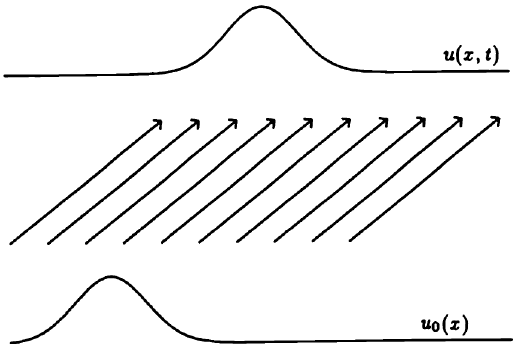
\includegraphics[width=\textwidth]{figures/charact_curves_linear_transport.png}
\caption{Characteristic curves for the linear advection equation.}
\label{fig:char_curve_sct1b}
\end{figure}
%
In the case of the 1-D Burger's equation, the eigenvalue is no longer constant and is equal to the solution itself $\lambda_2 = u(x,t)$. The slope of the characteristic curve is now a function of space and more precisely of the initial solution $u_0$ which requires us to analyze two distinct cases: a constant and a non-constant initial solution. In the former case, the slope of the characteristic is constant which is the same situation as with the linear advection equation previously discussed. In the latter case, the characteristic curves will not have the same slope and thus, may intersect. When two characteristic curves intersect, it means that, at a given time and position, two values of the solution are allowed (each characteristic curve carries different initial values of the solution): the solution displays an infinite gradient also called shock wave as shown in \fig{fig:char_curve_bg_sct1b}. 
\tcr{how do we see the infinite gradient in the equation?}\tcb{You see it with the characteristic equation: two values of u at a given point x -> infinite gradient}
%
\begin{figure}[H]
\centering
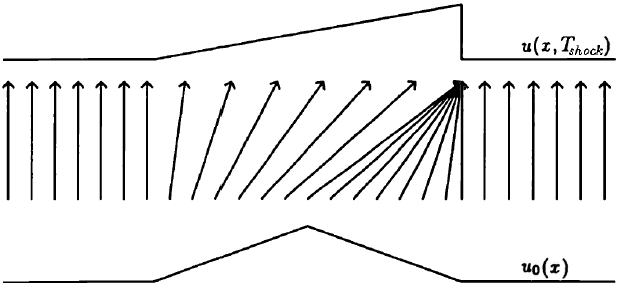
\includegraphics[width=\textwidth]{figures/shock_formation_burger.png}
\caption{Characteristic curves for the 1-D Burger's equation.}
\label{fig:char_curve_bg_sct1b}
\end{figure}
%
The time $T_{shock}$ at which the shock occurs can be analytically determined. Consider a 1-D non-linear flux $f(u)$ and two characteristic curves originating from the position $x_0$ and $x_0+dx$ carrying the initial values $u_0(x_0)$ and $u_0(x_0+dx)$, respectively. The characteristic curves are:
%
\begin{eqnarray}\label{eq:cc1_sct1b}
&&x_1(t) = x_0 + f'(u_0(x_0)) t \nonumber \\ 
&&x_2(t) = (x_0 + dx) + f'(u_0(x_0+dx)) t \, .
\end{eqnarray}
%
Now assume that the two characteristic curves intersect at time $T_{shock}$, which implies $x_1(T_{shock}) = x_2(T_{shock})$. Using \eqt{eq:cc1_sct1b} yields:
%
\begin{equation}\label{eq:cc1b_sct1b}
x_0 + f'(u_0(x_0)) T_{shock} = (x_0 + dx) + f'(u_0(x_0+dx)) T_{shock}
\end{equation}
%
From \eqt{eq:cc1b_sct1b}, after a few lines of algebra, an expression for $T_{shock}$ can be obtained: 
\begin{equation}\label{eq:cc2a_sct1b}
T_{shock} = \frac{-dx}{f'(u_0(x_0+dx))-f'(u_0(x_0))}
\end{equation} 
Taking the limit $dx \to 0$ and using the definition of the derivative, \eqt{eq:cc2a_sct1b} becomes:
\begin{equation}\label{eq:cc2_sct1b}
T_{shock} = \frac{-1}{f''(u_0) u_0'(x_0)} = \frac{-1}{f'(u_0(x_0))},
\end{equation} 
The trivial case $f''(u_0) = 0$ implies two options. The first case verifying $f''(u_0) = 0$ corresponds to a linear-flux which is ruled out since we assumed a non-linear flux. However, if one considers the linear advection equation, then $f''(u_0)=0$ and taking the limit of \eqt{eq:cc2_sct1b} yields $T_{shock} \to \infty$, which means that a shock wave never forms. This result is consistent with the conclusion made earlier in this section when studying the linear advection equation. The second case corresponds to a non-linear flux whose second-order derivative is locally zero. However, a shock occurs first where the derivative of the flux is negative to ensure positivity of $T_{shock}$, and its absolute value is maximum (so that $\frac{1}{f'(u_0)}$ is minimal). These conditions do not correspond to the case $f''(u_0) = 0$ which implies $f'(u_0) = 0$ locally \tcr{this is not clear, how does f''=0 implies f'=0?} and allow us to rule out the second case. Thus, the time of shock formation is:
%
\begin{equation}
T_{shock} = \frac{-1}{\min\left( f'(u_0) \right)} 
\end{equation}
% 
\tcr{that is not enough, $f''(u)0$ could be 0 at a given $x_0$. How can we modify this sentence?\\also, isn't the time of shock the minimum over all values of $x_0$?} \tcb{Is it better?} \tcr{not yet}
Once the shock is formed, at a time $t \geq T_{shock}$, more than two characteristic curves may intersect leading to a triple-valued situation as shown in \fig{fig:triple_pt_bg_sct1b}. 
%
\begin{figure}[H]
\centering
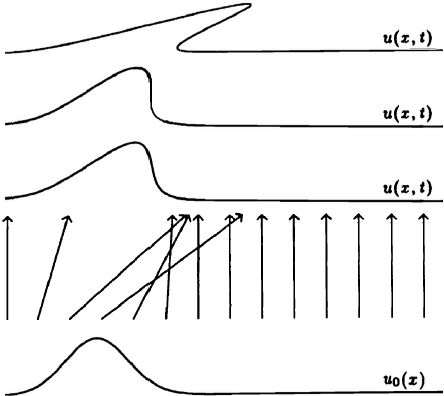
\includegraphics[width=\textwidth]{figures/charact_curves_burger.png}
\caption{Example of a triple-valued situation.}
\label{fig:triple_pt_bg_sct1b}
\end{figure}
%
In this case, uniqueness of the solution is not ensured since for a given position and time the solution admits three values. This particular phenomenon makes sense when solving the $3$-D shallow-water equations that are used to model a breaking wave on a sloping beach. However, when considering gas flows, uniqueness of the thermodynamic properties is required to ensure a point-wise single-valued density. From the last example, we understand that preventing the tripled-value situation from forming may be the key to obtaining the correct physical behavior when solving hyperbolic scalar equations and hyperbolic systems of equations (e.g., Euler equations). A solution to this problem could come from the study of an advection-diffusion equation type that is used, for instance, to model the propagation of particles in a material by both advection and diffusion phenomena. This type of equation is known to have unconditionally \emph{smooth solution} for all time and spatial location. A 1-D generic form is given in \eqt{eq:adv_diff_sct1b}.
%
\begin{equation}\label{eq:adv_diff_sct1b}
\partial_t u + \partial_x f(u) = \epsilon \partial_{xx} u \,,
\end{equation}
% 
where $\epsilon$ is a diffusion coefficient that can be solution-dependent in theory but is assumed constant for the purpose of this section. Since the main difference between the hyperbolic problem given in \eqt{eq:ivp_sct1b} and \eqt{eq:adv_diff_sct1b} lies in the diffusion term $\epsilon \partial_xx u(x,t)$, it is proposed to investigate its effect on the numerical solution. If the solution $u(x,t)$ is smooth, the diffusion term $\epsilon \partial_{xx} u(x,t)$ in \eqt{eq:adv_diff_sct1b} is negligible and the numerical solution is driven by the advection term $\partial_x f(u(x,t))$ so that \eqt{eq:adv_diff_sct1b} and \eqt{eq:ivp_sct1b} have similar behaviors. As the solution becomes steeper, the diffusion terms becomes large enough to influence the behavior of the numerical solution and will prevent the wave from breaking as it happens in hyperbolic problems. In other terms, the diffusion term, by monitoring the change of curvature in the numerical solution, locally affects the numerical solution where needed. The diffusion coefficient $\epsilon$ can be seen as a tuning coefficient that will also affect the smoothness of the numerical solution as shown in \fig{fig:epsilon}. As $\epsilon$ goes to zero, the numerical solution becomes sharper and tends to the solution obtained when solving the hyperbolic problem given in \eqt{eq:adv_diff_sct1b}. On the opposite, with a very large diffusion (viscosity) coefficient, the shock is smoothed out.
%
\begin{figure}[H]
\centering
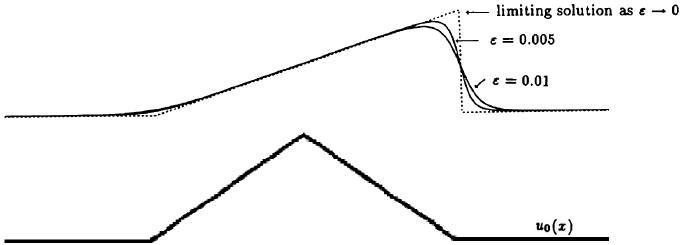
\includegraphics[width=\textwidth]{figures/effect_of_epsilon.png}
\caption{Influence of the viscosity coefficient $\epsilon$ on the numerical solution stiffness.}
\label{fig:epsilon}
\end{figure}
%
Thus, by adding a diffusion term, also called viscosity term, the numerical solution remains smooth and single valued, and should allow us to retrieve the correct physical behavior of a hyperbolic problem in the limit $\epsilon \to 0$. This approach is referred to as a \emph{vanishing viscosity method} and the numerical solution obtained with this method is denoted by $u^{\epsilon}(x,t)$. We can now define the notion of \emph{generalized solution}. 
%
\begin{definition}
\emph{
A generalized definition $u$ of a hyperbolic scalar equation conservation law 
\begin{equation}
\partial_t u + \div \mbold f(u) = 0, \nonumber
\end{equation}
is called an admissible vanishing viscosity solution if there is a sequence of smooth unique solutions $u^{\epsilon}$ to the parabolic equation 
\begin{equation}
\partial_t u^{\epsilon} +  \grad f(u^{\epsilon}) = \epsilon \nabla u^{\epsilon}, \nonumber
\end{equation}
that converges to $u$ as $\epsilon \to 0$.}
\end{definition}
%
It is now clear that by adding a viscosity term to an hyperbolic equation as previously explained, a generalized solution can be obtained with the vanishing viscosity approach. We will see in \sect{weak_sct1b} that a generalized solution can be also defined by the use of a mathematical technique resulting in a weak formulation of the hyperbolic scalar equation. Before doing so, it is proposed to investigate one more property of a shock wave: its speed. Knowing the breaking time $T_{shock}$ and position is not sufficient information to track a shock wave once it has formed. An useful information will be to derive an expression that provides us with the speed of the shock. One of the reasons for deriving such an expression is to obtain an analytical solution that can be used for comparison against numerical solutions in order to assess their accuracy. To do so, we consider, again, a general 1-D hyperbolic scalar equation for simplicity, as shown in \eqt{eq:rh_sct1b}:
%
\begin{equation}\label{eq:rh_sct1b}
\partial_t u(x,t) + \partial_x f(u(x,t)) = 0
\end{equation}
%
We assume that the position of the shock is given by a function of time denoted by $s(t)$ and that the associated speed is $S = \frac{ds}{dt}$. At this particular position, the derivatives of the solution $u$ and the flux $f(u)$ are no longer continuous. We also define a control volume $\left[ x_1; x_2 \right]$ that contains the shock wave so that $x_1 \leq s(t) \leq x_2$. \eqt{eq:rh_sct1b} is integrated over the control volume as shown in \eqt{eq:rh2_sct1b}:
%
\begin{equation}\label{eq:rh2_sct1b}
\frac{d}{dt} \int_{x_1}^{s(t)} u(x,t) dx + \frac{d}{dt} \int_{s(t)}^{x_2} u(x,t) dx + f(x_2,t) - f(x_1,t) = 0
\end{equation}
% 
The first two integrals can be recast by using the Leibnitz Rule:
%
\begin{equation}\label{eq:rh3_sct1b}
\frac{d}{dt} \int_{y_1(t)}^{y_2(t)} g(y,t) dy =  \int_{y_1(t)}^{y_2(t)} \frac{\partial g(y,t)}{\partial y} dy + g(y_2,t) \frac{d y_2(t)}{dt} - g(y_1,t) \frac{d y_1(t)}{dt} \,.
\end{equation}
% 
By noticing that $x_1$ and $x_2$ are fixed and thus not functions of time, we obtain:
%
\begin{equation}\label{eq:rh4_sct1b}
\int_{x_1}^{s(t)} \partial_t u(x,t) dx - \int_{s(t)}^{x_2} \partial_t u(x,t) dx + \left( u(s^-(t)) - u(s^+(t)) \right) S + f(x_2,t) - f(x_1,t) = 0 \,,
\end{equation}
%
where $u(s^-(t),t)$ and $u(s^+(t),t)$ are the values of the solution $u$ before and after the shock position, respectively. Assuming that the $x_1$ and $x_2$ approach the shock position $s(t)$ from the left and right, respectively, and that $\partial_t u$ is bounded, the two integrals vanish to yield the following expression for the shock speed  $S$:
%
\begin{equation}\label{eq:rh5_sct1b}
S = \frac{f(x_2,t) - f(x_1,t)}{u(s^-(t)) - u(s^+(t))} = \frac{\Delta f}{\Delta u} \,.
\end{equation}
%
The above expression for the speed of shock (\eqt{eq:rh5_sct1b}) is known as the Rankine-Hugoniot jump condition. The hyperbolic scalar equation given \eqt{eq:rh_sct1b} is only valid in smooth parts of the solution, and thus, require the use of the Rankine-Hugoniot jump condition in order to solve for the shock region.   

%===============================
\subsection{Weak solution and entropy condition}\label{weak_sct1b}
%===============================
As mentioned in \sect{sec:shock_form_sct1b}, another way to define a generalized solution is to use a mathematical technique that consists of multiplying the hyperbolic scalar equation by a smooth test function that is continuously differentiable within a compact support. Then, integration per parts is performed in order to transfer the derivative from the solution $u$ and onto the test function. The resulting equation involves fewer derivatives on $u$ and, hence, requires less smoothness. It is assumed that the test functions are only non-zero and continuously differentiable within a bounded set such as: $\phi(\mbold{r},t) \in C_0^1 \left( \mathbb{R}^d \times \mathbb{R^+} \right)$. 
Then, the 1-D conservation law $\partial_t u + \partial_x f(u) = 0$ is multiplied by the a test function $\phi(x,t)$ and integrated over space and time to yield:
%
\begin{equation}\label{eq:weak_sol_sct1b}
\int_0^{+\infty}\text{dt}\int_{-\infty}^{+\infty}\text{dx} \left[ \partial_t u(x,t) + \partial_x f(u) \right] \phi(x,t) = 0 \,.
\end{equation}
% 
Then, \eqt{eq:weak_sol_sct1b} is integrating by parts to obtain:
%
\begin{eqnarray}\label{eq:weak_sol2_sct1b}
\int_0^{+\infty}\text{dt}\int_{-\infty}^{+\infty}\text{dx} \left[ u(x,t) \partial_t \phi(x,t)   + f(u) \partial_x \phi(x,t)  \right] = \nonumber \\
-\int_{-\infty}^{+\infty}\text{dx} \phi(x,t) u(x,t) \left. \right|_0^{+\infty} - \int_0^{+\infty}\text{dt} \phi(x,t) f(u(x,t)) \left. \right|_{-\infty}^{+\infty}
\end{eqnarray}
%
where the two integrals on the right-hand-side of \eqt{eq:weak_sol2_sct1b} correspond to the boundary terms. Recalling that the test function is identically zero outside a bounded set which means $\phi(x,t) \to 0$ as $x \to \pm  \infty$ and $t \to +\infty$, \tcr{why does the test function depends on time and tends to 0 as time tends to infty?} \tcb{ I think it is for generality purpose. But the same derivation could be done with $\phi(x)$. In Leveque it is done with $\phi(x,t)$ p. 27 but they do not really justify this choice}\tcr{ok, please put the appropriate ref to Leveque's book, including the page number} all of the boundary terms vanish but for $t=0$. The resulting equation contains only one boundary term that is a function of the initial condition as shown in \eqt{eq:weak_sol3_sct1b}.
%
\begin{eqnarray}\label{eq:weak_sol3_sct1b}
\int_0^{+\infty}\text{dt}\int_{-\infty}^{+\infty}\text{dx} \left[ u(x,t) \partial_t \phi(x,t)   + f(u) \partial_x \phi(x,t)  \right] = \nonumber \\
-\int_{-\infty}^{+\infty}\text{dx} \phi(x,0) u_0(x) \,.
\end{eqnarray}
%
\eqt{eq:weak_sol3_sct1b} is used in the definition of a weak solution as follows:
%
\begin{definition}
\emph{The function $u(x,t)$ is called a weak solution of the conservative law
%
\begin{equation}
\partial_t u + \partial_x f(u) = 0, \nonumber
\end{equation}
%
if \eqt{eq:weak_sol3_sct1b} holds for all test functions $\phi(\mbold r, t) \in C_0^1 \left( \mathbb{R}^d \times \mathbb{R}^+ \right)$.}
\end{definition}
%
The formulation obtained in \eqt{eq:weak_sol3_sct1b} presents some similarities with the 1-D conservation law when integrated over a rectangle $\left[ x_1,x_2 \right] \times \left[ t_1,t_2 \right]$:
%
\begin{align}\label{eq:weak_sol4_sct1b}
\partial_t u(x,t) + \partial_x f(u) = 0 \to
\int_{x_1}^{x_2} \left[ x(x,t_2) - u(x,t_1) \right] dx + \int_{t_1}^{t_2} \left[ f(u(x_2,t)) - f(u(x_1,t)) \right]dt = 0
\end{align}
%
As a matter of fact, we can show that \eqt{eq:weak_sol3_sct1b} and \eqt{eq:weak_sol4_sct1b} are equivalent. To do so, we consider a test function $\phi(x,t)$ with the following properties:
%
\begin{equation}\label{eq:weak_sol5_sct1b}
\phi(x,t) = \left\{
\begin{array}{l}
1  \text{ for }  (x,t) \in \left[ x_1,x_2 \right] \times \left[ t_1,t_2 \right]  \\
0 \text{ for } (x,t) \notin \left[ x_1-\delta,x_2+\delta \right] \times \left[ t_1-\delta,t_2+\delta \right]
\end{array}\right.
\end{equation}
%
where $\delta$ is the width of the intermediate strip. Since the test function $\phi$ verifying \eqt{eq:weak_sol5_sct1b} vanish as $x \to \pm  \infty$ and $t \to \infty$, \eqt{eq:weak_sol3_sct1b} is still valid. The temporal and spatial derivatives of the test function $\phi(x,t)$ are zero everywhere but in the intermediate strip, and approach delta function as $\delta \to 0$. Thus, in the limit $\delta \to 0$, \eqt{eq:weak_sol3_sct1b} is shown to be equivalent to the integral form of the conservation law given in \eqt{eq:weak_sol4_sct1b}. A direct consequence of this result is that the weak solution in the sense of \eqt{eq:weak_sol3_sct1b} includes the solution of the hyperbolic conservation law we are seeking and also the vanishing viscosity generalized solution. However, uniqueness of the weak solution is not ensured by \eqt{eq:weak_sol3_sct1b} and can be demonstrated by considering a 1-D Riemann problem for a hyperbolic conservation law. The reader is referred to \cite{Toro} and \cite{Leveque} for additional details. The question arising from the previous statement is: how to identify the correct weak solution that corresponds to the physically vanishing viscosity solution? The answer lies in the entropy condition that is defined by analogy to the gas dynamics case. Mathematically, the entropy condition can be defined in multiple ways using either the speed of shock $S$ (see page 37 in \cite{Leveque}) or an entropy function that will be further detailed next. Because our focus is on hyperbolic system of equations, we have chosen to define the entropy condition through the derivation of an entropy residual for an hyperbolic conservation law. 

Before detailing the steps employed to obtain an entropy residual, we recall the meaning of the entropy condition for gas dynamics. In gas dynamics, the physical entropy is constant along a smooth path flow but experiences a jump to a higher value across a shock wave. Thus, the physical entropy is expected to increase if the flow contains a shock wave, which gives us a condition in order to pick out the correct weak solution. It remains to translate this condition into a mathematical statement. Before doing so, we want to emphasize the difference between the mathematical and physical entropies in order to clear any confusion. The physical entropy is by definition positive and increases as a function of time to reach a maximum value at steady-state. The mathematical entropy is defined convex and decreases as a function of time. In order to avoid any confusion, the mathematical and physical entropies will be referred to as $\eta$ and $s$, respectively. These two entropies are related to each other by the following relation:
%
\begin{equation}
s(u) = -\eta (u) + \eta_0 \,,
\end{equation}
%  
where $\eta_0$ is taken larger than the maximum of the absolute value of the mathematical entropy $\eta$ in order to ensure positivity of the physical entropy $s$. Of course, with such relation, convexity of $\eta$ implies that $s$ is concave. It is customary to work with the mathematical entropy when dealing with hyperbolic scalar equations, whereas the physical entropy is preferred for hyperbolic systems of equations such as the Euler equations. 

We now derive the entropy condition for a hyperbolic scalar conservation law of the generic form:
%
\begin{equation}\label{eq:weak_sol6bis_sct1b}
\partial_t u( \mbold{r}, t) + \div \mbold f(u) = 0 \,.
\end{equation}
%
We assume the existence of an entropy function $\eta(u)$ for which a conservation law to be determined holds. We first consider the case of a smooth flow and multiply \eqt{eq:weak_sol6bis_sct1b} by the derivative of $\eta$ with respect to $u$, denoted by $\eta_u$:
%
\begin{subequations}\label{eq:weak_sol6_sct1b}
\begin{equation}\label{eq:weak_sol6a_sct1b}
\eta_u \partial_t u( \mbold{r}, t) + \eta_u  \div \mbold f(u) = 0 \,.
\end{equation}
%
Using the chain rule, one obtains
%
\begin{equation}\label{eq:weak_sol6b_sct1b}
\eta_u \partial_t u( \mbold{r}, t) + \eta_u  \mbold f'(u) \cdot \grad u = 0 \,,
\end{equation}
%
which can be simplified to
%
\begin{equation}\label{eq:weak_sol6c_sct1b}
\partial_t \eta( u) +  \mbold f'(u) \cdot \grad \eta(u) = 0 \,.
\end{equation}
\end{subequations}
%
The relation given in \eqt{eq:weak_sol6c_sct1b} is a conservation law for $\eta$ which means that the mathematic entropy is conserved in a smooth flow. The entropy conservation law can also be recast as a function of the entropy flux $\mbold \psi$ by setting $\mbold \psi '(u) = \eta_u \mbold f'(u)$, which yields\footnote{here, $\eta$ depends only on $u$, so we could have written $\mbold \psi '(u) = \eta'(u) \mbold f'(u)$}:
%
\tcr{$\psi$ and $\mbold \psi$ look different, so when you want to denote a vector quantity, use the latter. For example, the equation need the bold. Check elsewhere as well}
\begin{equation}
\partial_t \eta( u) +  \div \psi(u) = 0 \,.
\end{equation}
%
The set $\left( \eta, \mbold \psi \right)$ is called an entropy pair. The corresponding physical entropy pair is $\left( s, -\mbold \psi \right)$ since $\mbold \psi '(u) = \eta_u \mbold f'(u)$.

\bigskip

We now consider a solution that presents one or more regions with a discontinuity or shock. The manipulations performed above are no longer valid since the solution is not smooth. Instead, it is proposed to look at the vanishing viscosity equation introduced in \eqt{eq:adv_diff_sct1b} and investigate the behavior of the weak solution as the viscosity coefficient tends to zero. Applying the vanishing viscosity method to \eqt{eq:weak_sol6_sct1b} yields
%
\begin{equation}\label{eq:weak_sol7_sct1b}
\partial_t u( \mbold{r}, t) + \div \mbold f(u) = \div \left( \mu( \grad u( \mbold{r}, t) \right) \,,
\end{equation}
%
where $\mu(\mbold r,t )$ is a positive viscosity coefficient that is typically spatially dependent in general. Because of the presence of the viscous term in \eqt{eq:weak_sol7_sct1b}, the solution remains smooth which allows us to perform the same manipulations as in \eqt{eq:weak_sol6_sct1b}. Hence, we obtain (the notation $( \mbold{r}, t)$ is dropped to simplify the derivation):
%
\begin{equation}\label{eq:weak_sol8_sct1b}
\partial_t \eta (u) + \div \mbold \psi (u) = \eta_u \div \left( \mu \grad u \right) \,,
\end{equation}
%
By integrating per parts the right-hand-side of \eqt{eq:weak_sol8_sct1b}, one obtains: 
%
\begin{equation}\label{eq:weak_sol9_sct1b}
\partial_t \eta (u) + \div \mbold \psi (u) =  \div \left( \eta_u \mu \grad u \right) - \mu( \grad u \cdot \grad \eta_u) \,.
\end{equation}
%
Since we are interested in the weak solution, \eqt{eq:weak_sol9_sct1b} is integrated over the space-time domain $\Theta = \left[ \mbold r_1,\mbold r_2 \right] \times \left[ t_1,t_2 \right]$ on the same model as in \eqt{eq:weak_sol4_sct1b}. It is also assumed that the shock remains within $\Theta$ for all time $t \in \left[ t_1, t_2 \right]$ and away from the boundaries. Thus, \eqt{eq:weak_sol9_sct1b} becomes:
%
\begin{eqnarray}\label{eq:weak_sol10_sct1b}
\int_{\mbold r_1}^{\mbold r_2}\text{d} \mbold r \int_{t_1}^{t_2} \text{dt} \left[ \partial_t \eta (u) + \div \mbold \psi (u) \right] &=&
\int_{\mbold r_1}^{\mbold r_2}\text{d} \mbold r \int_{t_1}^{t_2}\text{dt}  \div \left( \eta_u \mu \grad u \right)    \nonumber \\
&-& \int_{\mbold r_1}^{\mbold r_2}\text{d} \mbold r \int_{t_1}^{t_2} \text{dt} \mu \grad u \cdot \grad \eta_u \,.
\end{eqnarray}
%
The first term in the right-hand-side of \eqt{eq:weak_sol10_sct1b} can be recast as follows:
%
\begin{multline}\label{eq:weak_sol11_sct1b}
\int_{\mbold r_1}^{\mbold r_2}\text{d} \mbold r \int_{t_1}^{t_2} \text{dt} \div \left( \eta_u \mu \grad u \right) = \\
\int_{t_1}^{t_2} \text{dt} \left[ \eta_u \mu(\mbold r_2,t )\text{d} \mbold r \grad u( \mbold r_2,t) - \eta_u \mu(\mbold r_1,t ) \grad u( \mbold r_1,t) \right] \,.
\end{multline}
%
Since the shock position cannot be confounded with the boundary of the domain by assumption, the gradient of the solution at the points $\mbold r_1$ and $\mbold r_2$ remains bounded as $\mu \to 0$. Then, as the viscosity coefficient tends to zero, the whole integral vanishes. The second term in the right-hand-side of \eqt{eq:weak_sol10_sct1b} is more complex to deal with. First, the integral is recast by applying the chain rule to $\grad \eta_u$:
%
\begin{equation}\label{eq:weak_sol12_sct1b}
\int_{\mbold r_1}^{\mbold r_2}\text{d} \mbold r \int_{t_1}^{t_2}\text{dt} \mu \grad u \cdot \grad \eta_u = \int_{\mbold r_1}^{\mbold r_2}\text{d} \mbold r \int_{t_1}^{t_2}\text{dt} \mu\eta_{uu} \grad u \cdot \grad u \,,
\end{equation}
%
where $\eta_{uu}$ denotes the second derivative of $\eta$ with respect to $u$. As $\mu \to 0$, the integral does not vanish because of the terms $\grad u \cdot \grad u$ that will become larger and larger at the location of the discontinuity. However, by assuming that the entropy function is convex, i.e., $\eta_{uu} \geq 0$ and noticing that $\grad u \cdot \grad u \geq 0$ and $\mu \geq 0$, the sign of \eqt{eq:weak_sol12_sct1b} is found to be positive. Using the above results, we conclude that the vanishing viscosity weak solution satisfies the inequality:
%
\begin{equation}\label{eq:weak_sol13_sct1b}
\int_{\mbold r_1}^{\mbold r_2}\text{d} \mbold r \int_{t_1}^{t_2}\text{dt} \left[ \partial_t \eta (u) + \div \mbold \psi (u) \right] \leq 0,
\end{equation}
% 
for both smooth and discontinuous solutions.  Since the inequality given in \eqt{eq:weak_sol13_sct1b} holds for any $\Theta$, it can be simplified to
%
\begin{equation}\label{eq:weak_sol14_sct1b}
\partial_t \eta (u) + \div \mbold \psi (u) \leq 0
\end{equation}
%
in the weak sense and is known as the \emph{entropy inequality}. 
%
\begin{definition}
\emph{The function $u(\mbold r, t)$ is the entropy solution of the hyperbolic conservation law 
%
\begin{equation}
\partial_t u( \mbold{r}, t) + \div \mbold f(u) = 0 \nonumber
\end{equation}
%
if for all convex entropy pair $\left( \eta,\mbold \psi \right)$, the inequality 
%
\begin{equation}
\partial_t \eta (u) + \div \mbold \psi (u) \leq 0 \nonumber
\end{equation}
%
is satisfied in a weak sense.}
\end{definition}
%
The entropy inequality is used to analyze numerical methods in order to demonstrate that the numerical solution converges to the entropy solution. It is now proposed to see how the entropy inequality is used in the theoretical derivation of the entropy viscosity method for an hyperbolic scalar equation. 

%===============================
\subsection{Entropy Viscosity Method (EVM) and hyperbolic scalar equations}\label{sec:evm_hyp_sc_sct1b}
%===============================
This section aims at making the link between the theoretical results presented from \sect{sec:mat_ppr_sct1b} through \sect{weak_sct1b} and the entropy viscosity method (EVM) that is the focus of this dissertation. The results presented in this section rely on the work by Guermond et al. \cite{jlg1, jlg2, jlg3, valentin} and are used to familiarize the reader with the EVM.

In \sect{sec:shock_form_sct1b} and \sect{weak_sct1b}, we emphasized on the importance of ensuring uniqueness of the weak solution: this is achieved (i) by adding a viscosity term to the hyperbolic scalar equation in order to prevent triple-value points from forming and (ii) by using the entropy inequality (\eqt{eq:weak_sol14_sct1b}), which is mathematically equivalent to:
%
\begin{subequations}\label{eq:bg1_ev_sct1b}
%
\begin{equation}\label{eq:bg2_ev_sct1b}
\partial_t u + \div \mbold f(u) = \div \left( \mu \grad u \right)
\end{equation}
%
\begin{equation}\label{eq:bg3_ev_sct1b}
R(\mbold{r},t) = \partial_t \eta(\mbold{r},t) + \div \mbold \psi(\mbold{r},t) \leq 0,
\end{equation}
%
\end{subequations}
%
where $\mu(\mbold{r},t)$ is a spatially dependent viscosity coefficient and $R(\mbold{r},t)$ denotes the entropy residual. Assuming that $\mu$ is constant, \eqt{eq:adv_diff_sct1b} is retrieved. All of the other variables in \eqt{eq:bg1_ev_sct1b} were defined previously. It was shown in \sect{weak_sct1b} that the sign of the entropy residual, $R$, is related to the convexity of the mathematical entropy function $\eta$ and to the positivity of the viscosity coefficient $\mu(\mbold{r},t)$, when using the vanishing viscosity equation \eqt{eq:bg2_ev_sct1b}. Instead of taking a viscous flux of the form $\mu(\mbold{r},t) \grad u(\mbold{r},t)$ in \eqt{eq:bg2_ev_sct1b}, a more generic expression could have been assumed:
%
\begin{equation}
\partial_t u + \div \mbold f(u) = \div \mbold g (\mu, u), \nonumber
\end{equation}
%
where $\mbold g(\mu,u)$ is a viscous flux that will have to be determined such that $R$ is negative. In other words, the entropy condition could be used to derive the proper viscous terms that will ensure the correct sign for the entropy residual in the shock region. In the case of the hyperbolic scalar equations, the choice of the viscous term is obvious and probably unique. However, when considering hyperbolic systems of equations (e.g., Euler equations), deriving the viscous terms consistent with the entropy condition may no longer be evident. This aspect of the method is detailed in \sect{sec:hyp_sect1b}. 

Once the viscous term is derived and known to be consistent with the entropy condition, it remains to define the positive viscosity coefficient $\mu(\mbold{r},t)$. This step is crucial and should not be underestimated since it will determine the accuracy of the numerical method. We require the viscosity coefficient to be smooth: in \cite{Barter},  it is shown that a discontinuous viscosity coefficient could yield instabilities in the numerical solution. Such a behavior can be easily understood by considering the following example. Let us assume that the viscosity coefficient jumps from zero to a large value in the vicinity of the shock region. Because the dissipative term is conservative, the gradient of the solution, $\grad u$, will have to experience the same discontinuity as the viscosity coefficient, thus, yielding the same type of behavior in the solution itself. Going back to the definition of the $\mu$, the simplest definition we can think of is to set $\mu$ equal to a constant value. By doing so, dissipation will be added to the shock region, preventing the waves from breaking, but also to the smooth regions of the solution that do not need dissipation. Such a behavior is not ideal as it is over-dissipative. Another option would be to track the shock position in order to only add a significant amount of dissipation in the shock region.    
Defining a viscosity function capable of detecting and tracking shocks is not straightforward and needs to rely on a good understanding of the theory related to the formation of shocks. For example, we can think of monitoring the gradient of the solution itself that will become large in the shock region. Following this reasoning, a possible definition (in 1-D) would be to have $\mu(x,t) \propto \left| \partial_x u(x,t) \right|$. Another approach consists of using the entropy residual $R$ derived in \sect{weak_sct1b}. The entropy residual was initially studied to ensure uniqueness of the weak solution, but its variations are intimately related to the solution: $R$ is small as the solution is smooth and $R$ becomes large (in absolute value) in the shock region. Thus, by monitoring the variation of the entropy residual, the shock can be detected and also tracked. This approach was used by Guermond et al. \cite{jlg1, jlg2, jlg3} to solve for hyperbolic scalar equations such as the multi-D Burger's equation. Their method has been coined as the ``Entropy Viscosity Method'' (EVM). It requires the definition of three viscosity coefficients: a high-order viscosity coefficient, $\mu_e(\mbold{r},t)$, that is defined to be proportional to the absolute value of the entropy residual $\left| R\right|$,  a first-order viscosity coefficient, denoted by $\mu_{max}(\mbold{r},t)$ and set proportional to the local maximum eigenvalue of $\mbold{f}(u)$, and the final viscosity coefficient $\mu(\mbold{r},t)$ taken to be the minimum of the previous two coefficients, i.e., $\mu(\mbold{r},t) = \min \left( \mu_{max}(\mbold{r},t), \mu_e(\mbold{r},t) \right)$. The coefficient $\mu$ is the one actually used in the dissipative term $\div \left( \mu(\mbold{r},t) \grad u(\mbold{r},t) \right)$. The idea is to detect the entropy production characteristic of a shock wave. By defining $\mu_e(\mbold{r},t)$ proportional to $\left| R \right|$, the high-order viscosity will be large in the shock region and small elsewhere. The first-order viscosity serves as an upper bound for $\mu(\mbold{r},t)$ and its definition meets two criteria:
\begin{enumerate}
\item the definition of $\mu_{max}(\mbold{r},t)$ is determined so that the viscous regularization in \eqt{eq:bg2_ev_sct1b} is equivalent to the upwind-scheme when employing $\mu(\mbold{r},t) = \mu_{max}(\mbold{r},t) := \frac{h}{2} f'(u(\mbold{r},t))$ ($h$ being the local grid size). The derivation of the expression for $\mu_{max}$ can be found in \cite{jlg} and is easily demonstrated in 1-D when discretizing \eqt{eq:bg1_ev_sct1b} with a finite difference method (or equivalently with a continuous FEM methods with trapezoidal quadrature rules). 
\item the first-order viscosity coefficient is related to the Courant-Friedrichs-Lewy number (CFL) and more precisely to the stability of the numerical solution when using temporal explicit schemes.
\end{enumerate}
Based on the definition of the high- and first-order viscosity coefficients, the values taken by $\mu(\mbold{r},t)$ are as follows: when the solution is smooth, the entropy production measured by the entropy residual $R$ is small and thus $\mu(\mbold{r},t) = \mu_e(\mbold{r},t)$ is also small. In the shock region, the entropy residual is peaked and the high-order viscosity coefficient is expected to saturate to the first-order viscosity coefficient that is known to be over-dissipative since it is equivalent to the upwind scheme. With such definitions, the viscosity coefficient $\mu(\mbold{r},t)$ is peaked in the shock region and small elsewhere, while experiencing a continuous spatial variation. 

The definition of the high-order viscosity coefficient, $\mu_e$, is not complete yet. A dimensional analysis of \eqt{eq:bg1_ev_sct1b} shows that the viscosity coefficients have the units of $m^2 \cdot s^{-1}$, which yield the following definition for $\mu_e$:
%
\begin{equation}
\mu_e(\mbold{r},t) = h^2 \frac{\left| R(\mbold{r},t) \right|}{norm(s)} \nonumber
\end{equation}
%
where $norm(s)$ is a normalization function of the same unit as the entropy $s$. Guermond et al. proposed in \cite{jlg2} to use $norm(s) = || s - \bar{s} ||_\infty$ where $\bar{s}$ is the average value of the entropy function over the entire computational domain and $|| \cdot ||_\infty$ denotes the infinity norm. With such a normalization, $\mu_e$ was found to behave well in their numerical tests. Their definition of the EVM, when applied to hyperbolic scalar equation, is the following:
%
\begin{subequations}
%
\begin{equation}
\partial_t u + \div \mbold f(u) = \div \left( \mu \grad u \right)
\end{equation}
%
\begin{equation}
R = \partial_t \eta + \div \mbold \psi
\end{equation}
%
\begin{equation}\label{eq:evm_def_sct1b}
\left\{
\begin{array}{l}
\mu(\mbold{r},t) = \min \left( \mu_e(\mbold{r},t), \mu_{max}(\mbold{r},t) \right) \\
\mu_{max}(\mbold{r},t) = \frac{h}{2} \left| f'(u(\mbold{r},t)) \right| \\
\mu_e(\mbold{r},t) = h^2 \frac{\max \left(\left| R(\mbold{r},t), J \right) \right|}{|| s - \bar{s} ||_\infty}
\end{array}
\right.
\end{equation}
%
\end{subequations}
%
The jump of the entropy flux $\mbold \psi$, denoted by $J$, is included in the definition of the high-order viscosity coefficient since it is also a good indicator of entropy production. Information relative to the computation of the jump with a continuous Galerkin finite element method (CGFEM) discretization will be detailed in \sect{sec:spatial_discretization}. In the case of discontinuous schemes, the reader is referred to \cite{valentin}. Numerical results for the multi-D Burger's equation solved with the EVM  and discretized using the CGFEM are presented in \sect{sec:burger_sct2b}.
%
\begin{remark}
The definition of the viscosity coefficients given in \eqt{eq:evm_def_sct1b} requires an isentropic mesh in order to be able to define the grid size $h$. An alternative definition without $h$ is under investigation for the case of hyperbolic scalar equations.
\tcr{not true; if you if you define $\mu$ per cell $K$, then you can use $h_K$, the diameter of cell $K$ in multi-D, and then you do not need to require mesh uniformity. This may be a detail but your remark is not necessarily 100\% true} \tcb{Is it better or am I still missing something?} \tcr{I do not understand why you say isentropic mesh. I changed that to uniform mesh but you changed it back to isentropic. What is an isentropic mesh?}
\end{remark}


%%%%%%%%%%%%%%%%%%%%%
\section{Hyperbolic system of equations}\label{sec:hyp_sect1b}
%%%%%%%%%%%%%%%%%%%%%
In this section, the entropy viscosity method is applied to non-linear hyperbolic systems of equations. The reader can refer to \cite{Toro} and \cite{Leveque} for an extension of the theoretical notions (eigenvalues, characteristic curves, $\ldots$) in the case of non-linear hyperbolic conservation laws. The objective of this section is to provide the reader with a methodology on how to apply the EVM to any hyperbolic system of equations. For academic purpose, we will rely on the latest published version of the EVM \cite{valentin} for the multi-D Euler equations in order to understand the main steps of the method. Other more recent publications will be also used. \cite{jlg, jlg2} are good prerequites to \cite{valentin} to observe the evolution of the EVM in the recent years. For hyperbolic system of equation, it is customary to work with the physical entropy $s$ that is of opposite sign of the mathematical entropy $\eta$.\\

To the best of our knowledge, the EVM was successfully applied to one hyperbolic system of equation: the multi-D Euler equations with the ideal gas equation of state \cite{jlg, valentin}. Good agreements with the exact solutions were obtained in 1- and 2-D results when using discontinuous schemes (finite volume and discontinuous Galerkin finite element methods), spectral and Fourier methods. We now recall the details of the latest version of the method \cite{valentin} and remind the reader that this version will be used as a starting point and modified during this dissertation. The viscous regularization derived from the entropy condition for the multi-D Euler equations with the ideal gas equation of state is as follows:
%
\begin{subequations}\label{eq:euler_visc_sct1b}
%
\begin{equation}
\partial_t \rho + \div \left( \rho \vec{u} \right) = \div \left( \mu \grad \rho \right) 
\end{equation}
%
\begin{equation}
\partial_t \left( \rho \vec{u} \right) + \grad \left( \rho \vec{u} \otimes \vec{u} \right) + \grad P = \div \left( \rho \mu \grad^s \vec{u} \right)
\end{equation}
%
\begin{equation}
\partial_t \left( \rho E \right) + \div \left[ \vec{u} \left( \rho E +P \right) \right] = \div \left( \kappa \vec{u} \grad^s \vec{u} + \kappa \grad T \right)
\end{equation}
%
\begin{equation}\label{eq:eos_sct1b}
P = \left( \gamma-1 \right) \rho e = \left( \gamma-1 \right) C_v \rho T
\end{equation}
%
\end{subequations}
%
where $\rho$, $\rho \vec{u}$ and $\rho E $ are the fluid density, momentum and total energy, respectively, and will be referred to as the conservative variables. The pressure $P$ and the temperature $T$ are computed from the Ideal 
Gas equation of state (IGEOS) recalled in \eqt{eq:eos_sct1b} which is a function of the density $\rho$ and the specific internal energy $e$. The heat capacity $C_v$ is constant by definition. The viscosity coefficients $\mu$ and $\kappa$ are space- and time-dependent and are taken proportional to an entropy residual $R$ as follows:
% 
\begin{subequations}
%
\begin{equation}
\left\{
\begin{array}{l}
\mu\left( \mbold{r},t \right) = \min \left( \mu_e\left( \mbold{r},t \right), \mu_{max}\left( \mbold{r},t \right) \right) \\
\kappa\left( \mbold{r},t \right) = \frac{\gamma \Pr}{\gamma-1} \mu\left( \mbold{r},t \right),
\end{array}
\right.
\end{equation}
and
\begin{eqnarray}\label{eq:visc_def_sct1b}
&&\mu_{max}\left( \mbold{r},t \right) = \frac{h}{2} \left( ||\vec{u}\left( \mbold{r},t \right)|| + c\left( \mbold{r},t \right)  \right) \nonumber \\
&&\mu_e\left( \mbold{r},t \right) = C_E h^2 \frac{\max \left( \left|| R\left( \mbold{r},t \right) \right|, J \right)}{|| s\left( \mbold{r},t \right) - \bar{s}(t) ||_\infty} \\
&&R\left( \mbold{r},t \right) = \partial_t s\left( \mbold{r},t \right)  + \vec{u} \cdot \grad s\left( \mbold{r},t \right), \nonumber
\end{eqnarray}
%
\end{subequations}
%
where $C_E$ is a constant coefficient of order one, $h$ is the grid size, $c = \sqrt{\gamma P / \rho}$ is the speed of sound and $\Pr$ is a Prandtl number taken in the interval $\in \left[ 0; \frac{1}{4} \right]$. The variable $J$ denotes the jump of the entropy flux $\vec{u} s$, is cell-wise constant, and is computed at the interfaces between a cell and its direct neighbors \cite{valentin}. The entropy $s$ is function of the density and the pressure:
%
\begin{equation}
s\left( \rho, P \right) = C_v \ln \left( \frac{P}{\rho^\gamma} \right),
\end{equation}
%
but can also be recast as a function of the density and the internal energy using the IGEOS. The symmetric gradient $\grad^s \vec{u}$ is defined with the following entries $\grad^s \vec{u}_{i,j} = \frac{1}{2} \left( \frac{\partial u_i}{\partial x_j}+\frac{\partial u_j}{\partial x_i} \right)$. The current definition of the EVM suffers from a few  theoretical gaps. The normalization parameters $|| s\left( \mbold{r},t \right) - \bar{s}(t) ||_\infty$ used in the definition of the high-order viscosity coefficient $\mu_e$ in \eqt{eq:visc_def_sct1b} does not currently have a theoretical justification beyond a dimensionality argument. The same remark can be made for the Prandtl number that is set by the user based on testing and experience. Moreover, the viscous regularization given in \eqt{eq:euler_visc_sct1b} depends on the euqation of state and, as given here, is only valid for the IGEOS. However, new developments in the theory extended the validity of the method for the multi-D Euler equations to any equation of state \cite{jlg} and hence makes it a good candidate for nuclear reactor applications, for instance. Thus, based on the work done in \cite{jlg} and with the experience gained from \cite{jlg2, valentin} the following methodology is proposed. We consider the generic non-linear hyperbolic system in order to explain the methodology:
%
\begin{equation}\label{eq:hyp_syst_sct1b}
\partial_t \boldsymbol{U} + \div \boldsymbol{F} \left( \boldsymbol{U} \right) = 0,
\end{equation}
%
where $\boldsymbol{U} = \left( U_1, \dots, U_n \right)$ is the solution vector and $\boldsymbol{F} \left( \boldsymbol{U} \right) = \left( F_1, \dots, F_n \right)$ is a hyperbolic flux whose eigenvalues are denoted by $\left( \lambda_1, \dots, \lambda_n \right)$.
\begin{enumerate}
\item The first step consists of deriving a conservation law for an entropy function denoted by $s\left(\boldsymbol{U}\right)$ of the form: 
%
\begin{equation}
R\left(\boldsymbol{U}\right) = \partial_t s\left(\boldsymbol{U}\right) + \boldsymbol{F}_{\boldsymbol{U}} \cdot \grad s \left(\boldsymbol{U}\right) = 0,
\end{equation}
%
where $\boldsymbol{F}_{\boldsymbol{U}} = \frac{\partial \boldsymbol{F}}{\partial \boldsymbol{U}}$ is the jacobian matrix of the hyperbolic flux $\boldsymbol{F} \left( \boldsymbol{U} \right)$.
This entropy equation/residual is obtained from the hyperbolic system of equation given in \eqt{eq:hyp_syst_sct1b} either by multiplying by the matrix $s_{\boldsymbol{U}} = \frac{\partial s (\boldsymbol{U})}{\partial \boldsymbol{U}}$ and using the chain rule, or by doing combination of the equations of the hyperbolic system. This step is well documented for the multi-D Euler equation \cite{Toro}. The objective is to understand the steps that lead to the derivation of the entropy equations since the same steps will be used to obtain the viscous terms.
\item We now want to derive the viscous terms consistent with the entropy condition. The method is inspired of what is done for the multi-D Euler equations in \cite{jlg}. To do so, we first modify \eqt{eq:hyp_syst_sct1b} by adding a viscous flux $\boldsymbol{G} \left( \boldsymbol{U} \right)$ that we want to determine by invoking the entropy inequality:
%
\begin{equation}\label{eq:hyp_syst2_sct1b}
\partial_t \boldsymbol{U}(\mbold{r},t) + \div \boldsymbol{F} \left( \boldsymbol{U} \right) = \div \boldsymbol{G} \left( \boldsymbol{U} \right),
\end{equation}
%
Then, the entropy residual is derived again:
%
\begin{eqnarray}\label{eq:hyp_syst3_sct1b}
R\left(\boldsymbol{U}\right) = \partial_t s\left(\boldsymbol{U}\right) + \boldsymbol{F}_{\boldsymbol{U}} \cdot \grad s \left(\boldsymbol{U}\right) &=& s_{\boldsymbol{U}} \div \boldsymbol{G} \left( \boldsymbol{U} \right) \nonumber \\
R\left(\boldsymbol{U}\right) = \partial_t s\left(\boldsymbol{U}\right) + \boldsymbol{F}_{\boldsymbol{U}} \cdot \grad s \left(\boldsymbol{U}\right) &=& \nonumber \\
\div ( s_{\boldsymbol{U}} \boldsymbol{G}  \left( \boldsymbol{U} \right) ) &-& \boldsymbol{G}  \left( \boldsymbol{U} \right) \cdot \grad s_{\boldsymbol{U}}.
\end{eqnarray}
%
To prove that the entropy residual $R$ remains positive, the non-conservative terms of the right hand-side have to be positive. Thus, positivity of the entropy residual is tied to the definition of the viscous term $\boldsymbol{G}  \left( \boldsymbol{U} \right)$ and the entropy function $s$. For the multi-D Euler equation, Guermond et al. \cite{jlg} proved that the entropy function $s$ needs to be concave ($-s$ is convex) in order to ensure positivity of the entropy residual for any equation of state. This condition is tied to a particular choice of the dissipative terms that will be detailed in \sect{sec:entro_visc} and to the positivity of the viscosity coefficients. In the general case, the parabolic regularization \cite{Parabolic} can be used and consists of dissipating on the solution itself  $\boldsymbol{U}$ as shown in \eqt{eq:hyp_syst4_sct1b}: 
%
\begin{equation}\label{eq:hyp_syst4_sct1b}
\partial_t \boldsymbol{U}(\mbold{r},t) + \div \boldsymbol{F} \left( \boldsymbol{U} \right) = \div \left( \mu \grad \left( \boldsymbol{U} \right) \right),
\end{equation}
%
where $\mu$ is a positive viscosity coefficient. \eqt{eq:hyp_syst4_sct1b} obeys to the entropy condition under the condition of having a concave entropy $s$ \cite{Parabolic}. Using the entropy condition, other viscous regularizations can be found with multiple viscosity coefficients (see \cite{jlg} for Euler equations). However, it is expected that they all degenerate to the parabolic regularization when assuming that all viscosity coefficients are equal to each other. Furthermore, for consistency with the parabolic regularization \cite{Parabolic}, the entropy function $s$ is required to be concave. In other terms, the parabolic regularization can be used as a hint in order to derive a viscous regularization with multiple viscosity coefficients. We will see in \sect{sec:lowMach} that having a viscous regularization with two viscosity coefficients is required for the multi-D Euler equation in order to have well-scaled viscous terms in the non-isentropic low-Mach limit. Before moving forward to the next step, we recast the entropy residual $R$ as a function of the conservative variables. This step is justified by the difficulty encountered in obtaining an analytical expression for the entropy function. This is particularly true for Euler equations when dealing with equation of states. We assume that the entropy residual was successfully recast as a function of the conservative variables and that the new entropy residual is denoted by $\tilde{R}$. The reader is referred to \sect{sec:new_ent_prod} for an example.
\item Once the entropy residual is proven to be positive, it remains to define the viscosity coefficient(s). Assuming that a viscous regularization was derived in step 2 with $n$ viscosity coefficients denoted by $\mu_i$, $i\in \left[1, \dots, n\right]$, a general definition can be given in the form:
%
\begin{equation}
\left\{
\begin{array}{l}
\mu_i(\mbold{r},t) = \max \left( \mu_{i,e}(\mbold{r},t), \mu_{max}(\mbold{r},t) \right) \nonumber \\
\mu_{max}(\mbold{r},t) = \frac{h}{2} \max_{i\in \left[1,n\right]} |\lambda_i(\mbold{r},t)| \nonumber \\
\mu_{i,e}(\mbold{r},t) = h^2 \frac{\max\left(\tilde{R}(\mbold{r},t), J\right)}{norm_i(\mbold{r},t)}, \nonumber
\end{array}
\right.
\end{equation}
%
where $\mu_{e,i}$ and $\mu_{max}$ are the high- and first-order viscosity coefficients, respectively. The high-order viscosity coefficient $\mu_{e,i}$ is defined proportional to the local entropy residual $R(\mbold{r},t)$ and also function of a normalization parameter $norm_i(\mbold{r},t)$ that will be explained further. The first-order viscosity coefficient $\mu_{max}(\mbold{r},t)$ is set proportional to the maximum eigenvalue and is unique for all viscosity coefficients $\mu_i(\mbold{r},t)$. $h$ still denotes the local grid size. In order to have a complete definition for the $\mu_e(\mbold{r},t)$, the normalization parameter $norm_i(\mbold{r},t)$ needs to be defined. It is well known that hyperbolic system of equations suffer from ill-scaled dissipative term in some particular asymptotic limit. This is particularly true for the stabilization methods used for the multi-D Euler equations, that require a fix in the low Mach asymptotic limit in order to yield the correct asymptotic behavior \cite{LowMach1, LowMach2}. Thus, by non-dimensionalizing the equations, the normalization parameter $\norm_i(\mbold{r},t)$ may be determined for each viscosity coefficients $\mu_i(\mbold{r},t)$ to ensure well-scaled dissipative terms. 
%\item We are also interested in solving hyperbolic system of equations with source terms for nuclear reactor applications, which requires to study the effect of the source terms on the entropy residual $R$. It is expected that the steps in the derivation of the entropy residual will remain the same, but extra terms will appear because of the physical source terms. We will need to determine how these additional terms will affect the sign of the entropy residual and modify the definition of the high-order viscosity coefficient accordingly. 
\end{enumerate}
This three-step process is applied to the multi-D Euler equations with variable area in \chap{chap:euler}, to the seven-equation model in \chap{chap:seven} and to the radiation-hydrodynamic equations in \chap{chap:hydro} to determine the viscous terms and to define the viscosity coefficients. Details about the implementation of the EVM with continuous Galerkin finite element method are provided in \sect{sec:spatial_discretization}. The jump $J$ is given on a case by case basis since its definition depends on the variables involved in the expression of the new entropy residual $\tilde{R}$.
%\item hyperbolic system of equations can also produce shocks.
%\item same treatment as scalar equations.
%\item Lapidus, pressure-based ...
%\item low Mach
%\item 
%\end{itemize}
%%%%%%%%%%%%%%%%%%%%%